\chapter{Geant4 simulation} \label{sec:geant4}
In this thesis, the Monte Carlo simulation was employed Geant4.10.01.p01 toolkit with the QGSP\_BERT\_HP physics package.
This physics package adopts precompound model for high energy hadrons ($10-25 GeV/c$)which are protons, neutrons, pions, kaons and nuclei and Bertini cascade for low energy hadrons ($\sim 10GeV/c$).
HP means high precision for the neutron espacially thermal neutron ($<20MeV/c$), so these neutrons were transported by the high precision data.

The purposes of Monte Carlo are evaluation of the acceptance of the CDS and estimation of contribution from specific reactions.
1-step reactions was simulated using previous experimental data of $\bar{K}N$ scattering and fermi momentum, which was used to evaluate contamination to 2-step reactions in this thesis.
Also, 2-step reactions was simulated as $S$-wave scattering, which was used to evaluated the acceptance of the CDS.
In $d(K^-, n \pi^+ \pi^-)"n"$ final state, 2-step simulation of $d(K^-, n)"\pi^{\mp}\Sigma^{\pm}$ was used to separation of each modes by template fittings.
As Sec\ref{sec:tempfit}, this final state was sucessfully decomposed to 5 reactions which are $K^- d \rightarrow \pi^{\mp}\Sigma^{\pm} n$ (1-step), $K^-d\rightarrow K^0 n n$ (1-step)
and $K^-d\rightarrow n \pi^{\mp}\Sigma^{\pm}$ (2-step).

The result of the Monte Carlo simulation of $d(K^-, n \pi^+ \pi^-)"n"$ final state and template fitting was used for some calibrations.
The CDS magnetic field was calibrated using $K^0$ peak which was subtracted background which was shown in Fig\ref{fig:K0_wFit}.
We searched correct field value value while changing the inputed field value that indicates in Fig\ref{fig:CDS_field}.
The CDC resolution was estimated at $280\mu m$ using width of $K^0$ peak while changing the inputed resolution.

The NC resolution was evaluated $d(K^-, n \pi^+ \pi^-)"n"$ peak which was shown in Fig\ref{fig:NC_reso}.
The $K^- d \rightarrow n \pi+ \pi^- n$ events was decomposed which described in Sec\ref{sec:tempfit},
so red plot in Fig\ref{fig:NC_reso} was reproduced using the Monte Carlo samples and template fitting.
The NC time resolution was estimated at $170 ps$ while changing the inputed resolution for the Monte Carlo simulation.
The PC/CVC time resolution is adopted similar procedure to $d(K^-, p \pi^- \pi^-)"p"$ peak which is come from the $K^- d \rightarrow p \Lambda \pi^-$ scattering as shown in Fig\ref{fig:FP_reso}.

The $d(K^-, n)"X"$ missing mass resolution was estimated using the $d(K^-, n)"\pi^{\mp}\Sigma^{\pm}"$ Monte Carlo simulation as shown in Fig\ref{fig:KN_MM_reso},
so we estimated about $10MeV/c^2$ at the $\bar{K}N$ threshold.
The resolution was given 3rd polynomial function by fitting to this figure which was shown in same figure.

\begin{figure}[htbp]
  \centering
  \begin{tabular}{cc}
    \begin{minipage}{0.5\hsize}
      \includegraphics[width=5cm]{../pic/Dron/K0_peak_wBG.eps}
    \end{minipage}
    \begin{minipage}{0.5\hsize}
      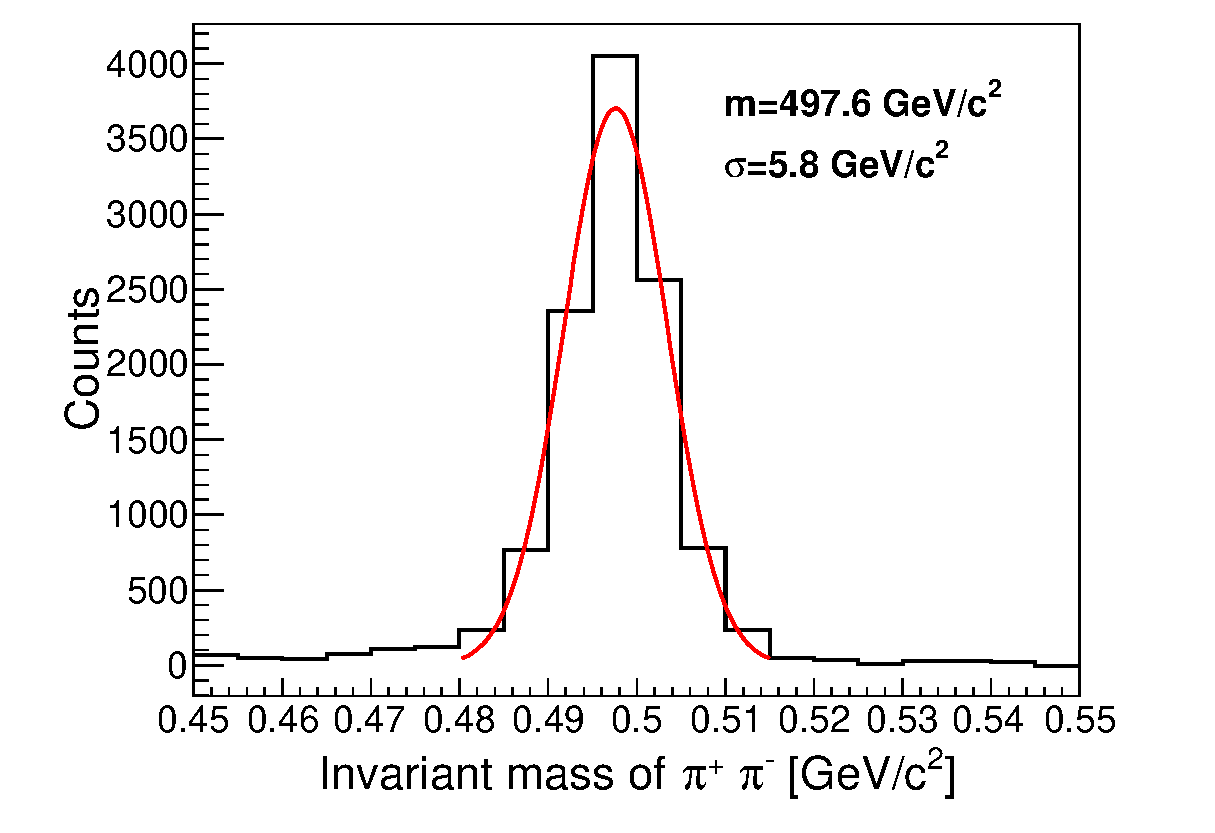
\includegraphics[width=5cm]{../pic/Dron/K0_peak_wFit.eps}
    \end{minipage}
  \end{tabular}
  \caption{
    Right figure shows the invariant mass of $\pi^+ \pi^-$ in the $d(K^-, n \pi^+ \pi^-)"n"$ missing masses with estimated background which was indicated as gray line.
    Left figure shows the $K^0$ peak which was subtrackted spectrum with fitted Gaussian, that was red line.
  }
  \label{fig:K0_wFit}
\end{figure}

\begin{figure}[htbp]
  \centering
  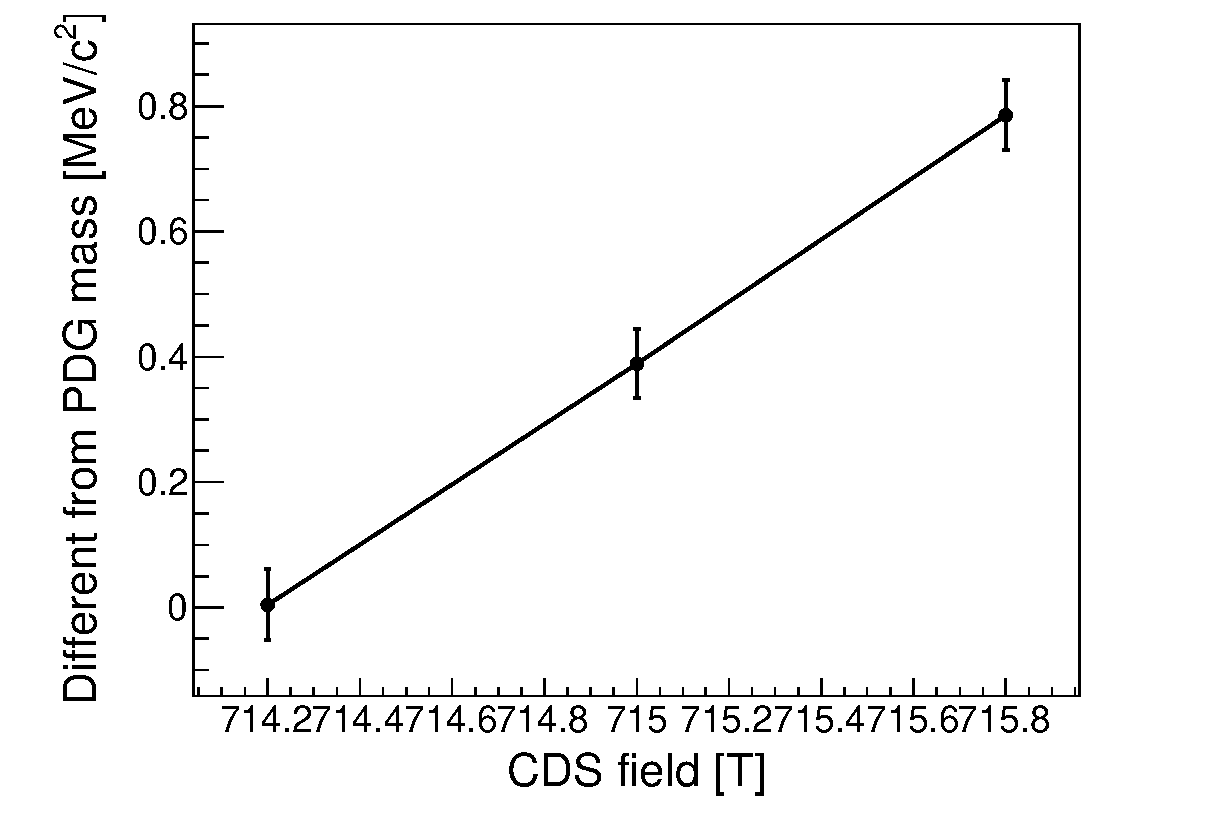
\includegraphics[width=8cm]{../pic/Dron/CDC_field.eps}
  \caption{
    This figure indicates relation of the CDS field value and $K^0$ peak position which was indicated in left figure of Fig\ref{fig:K0_wFit}.
  }
  \label{fig:CDS_field}
\end{figure}

\begin{figure}[htbp]
  \centering
  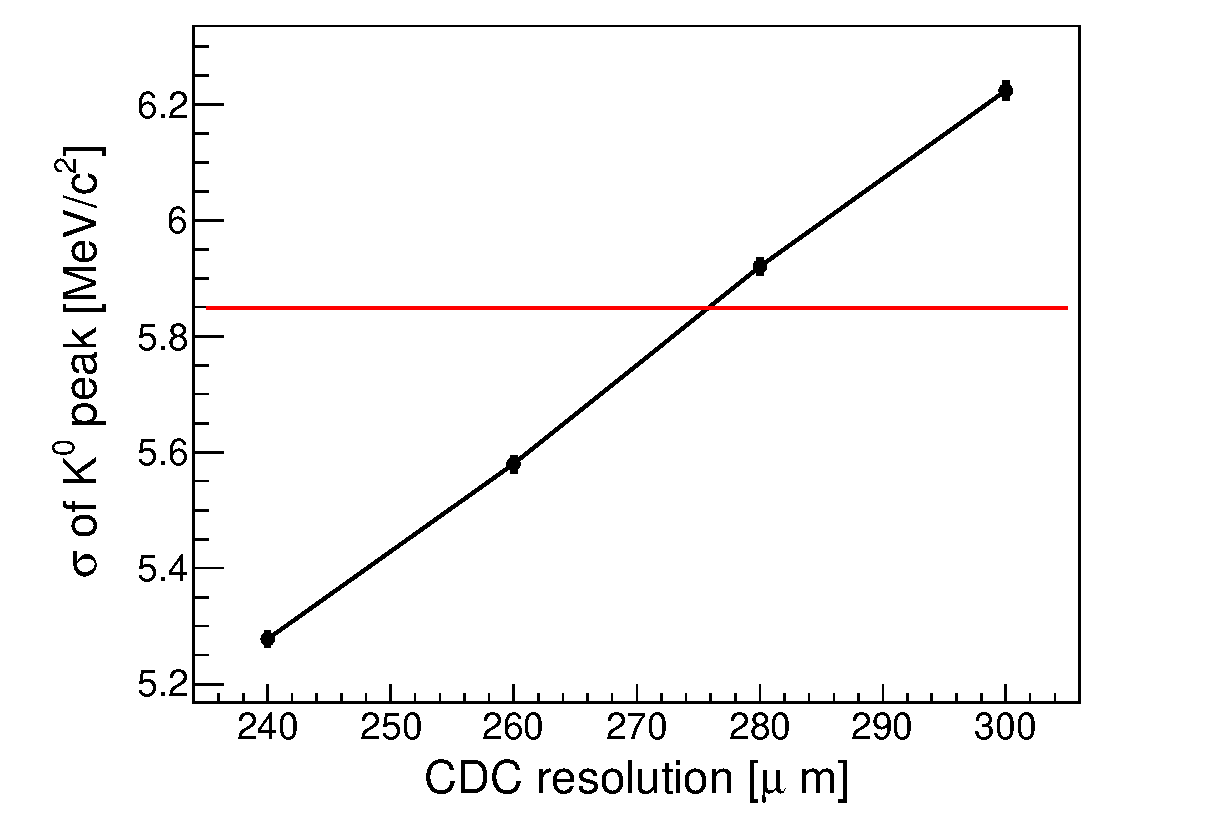
\includegraphics[width=8cm]{../pic/Dron/CDC_reso.eps}
  \caption{
    This figure indicates relation of the CDC resolution and width of $K^0$ peak.
    Red line indicates width of $K^0$ peak by data
    which was discribed in left figure of Fig\ref{fig:K0_wFit}.
  }
  \label{fig:CDC_reso}
\end{figure}

\begin{figure}[htbp]
  \centering
  \begin{tabular}{cc}
    \begin{minipage}{0.5\hsize}
      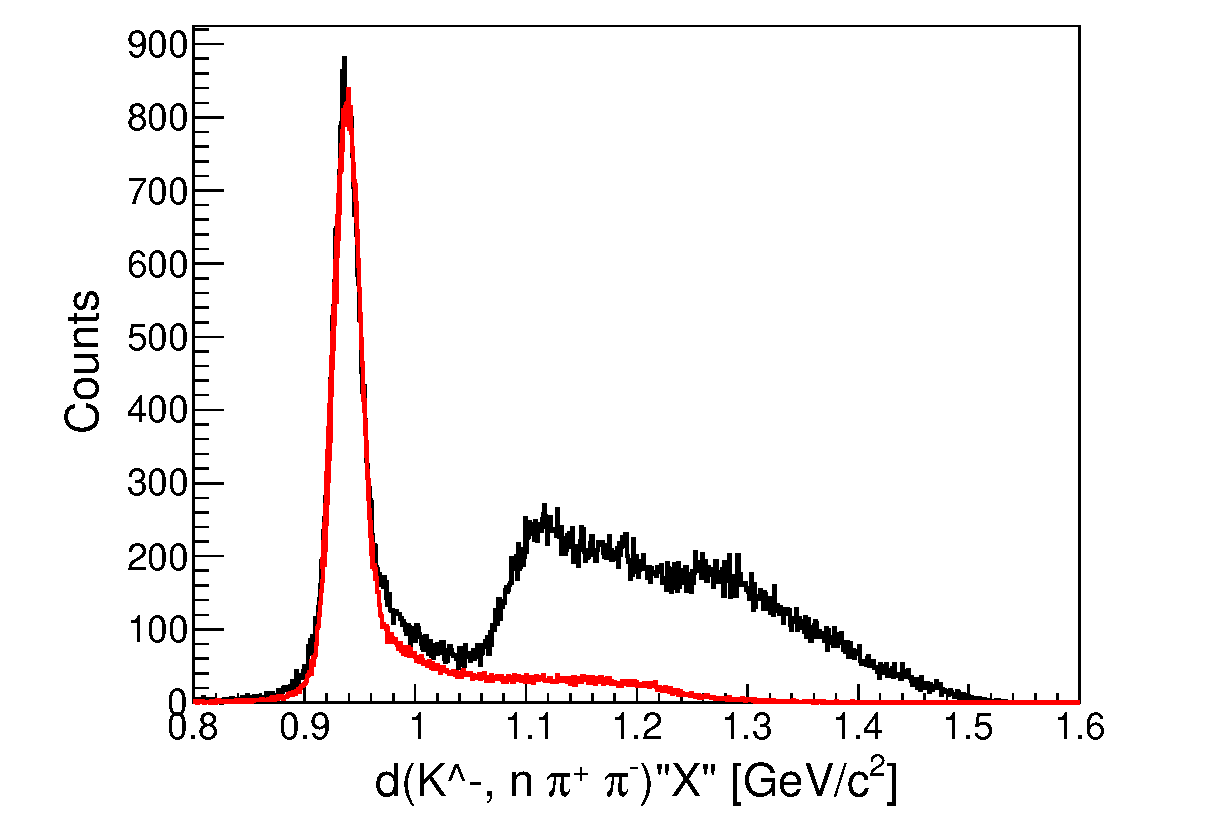
\includegraphics[width=7cm]{../pic/Dron/NC_reso_raw.eps}
    \end{minipage}
    \begin{minipage}{0.5\hsize}
      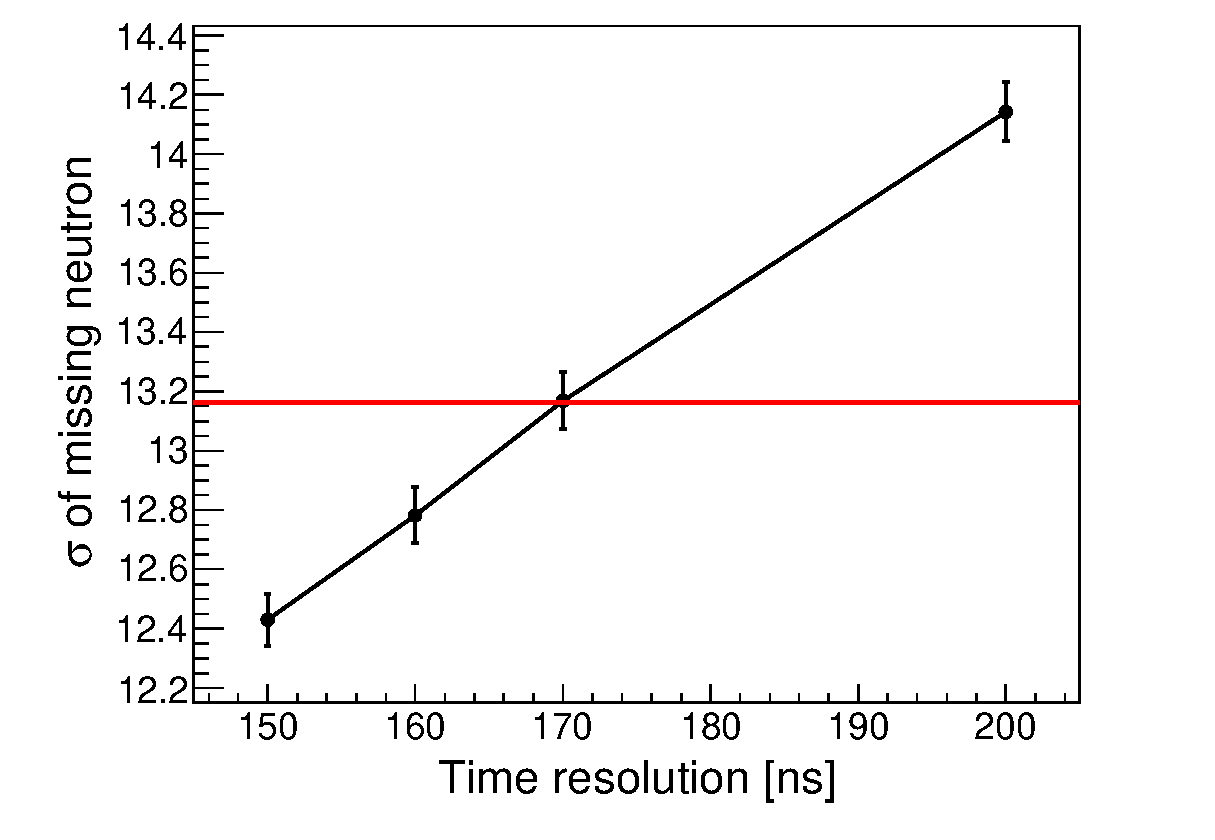
\includegraphics[width=7cm]{../pic/Dron/NC_reso.eps}
    \end{minipage}
  \end{tabular}
  \caption{
    Left figure shows $d(K^-, n \pi^+ \pi^-)"n"$ missing mass spectra. Black one indicates data and red one indicates the summed up Monte Carlo simulation datas.
    Right figure indicates relation of $\sigma$ of $d(K^-, n \pi^+ \pi^-)"n"$ peak which was estimated Gaussian fitting and inputed time resolution.
    Red line indicate fitting result of the data.
  }
  \label{fig:NC_reso}
\end{figure}

\begin{figure}[htbp]
  \centering
  \begin{tabular}{cc}
    \begin{minipage}{0.5\hsize}
      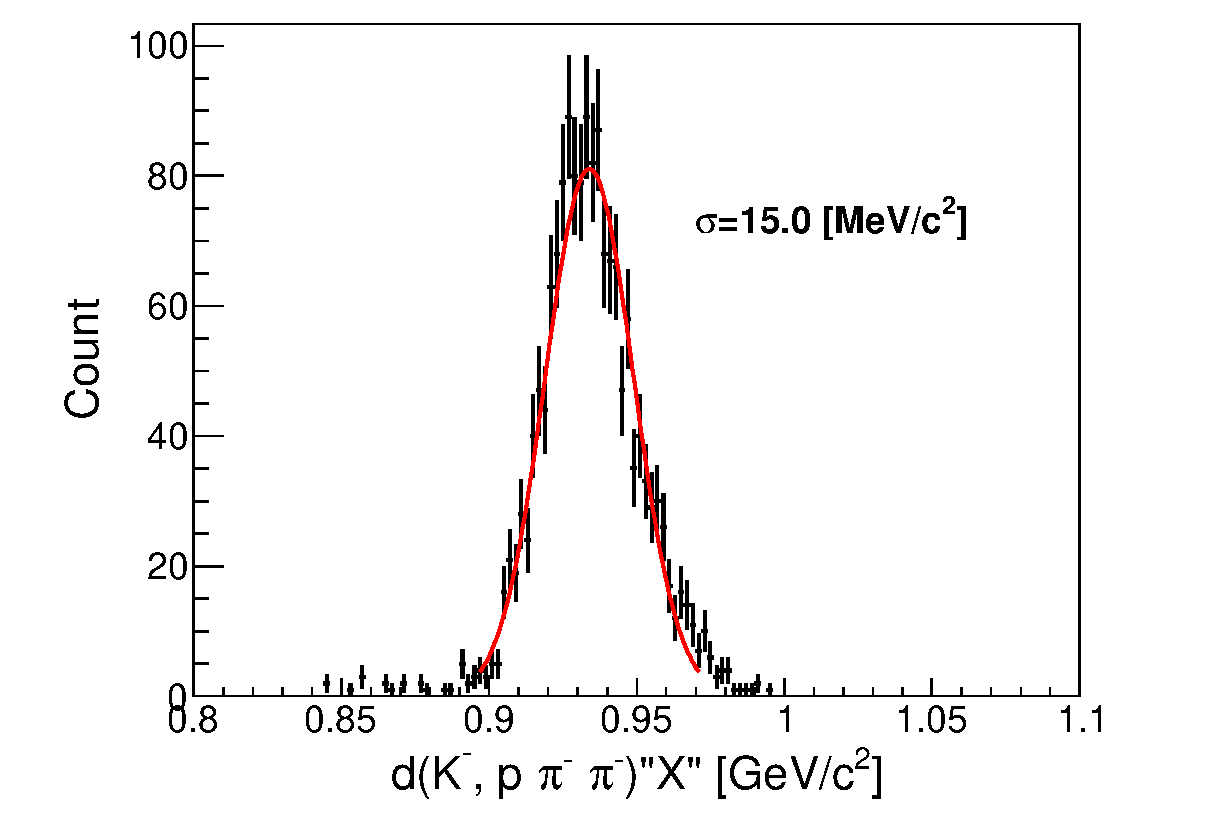
\includegraphics[width=7cm]{../pic/Dron/KP_reso_data.eps}      
    \end{minipage}
    \begin{minipage}{0.5\hsize}
      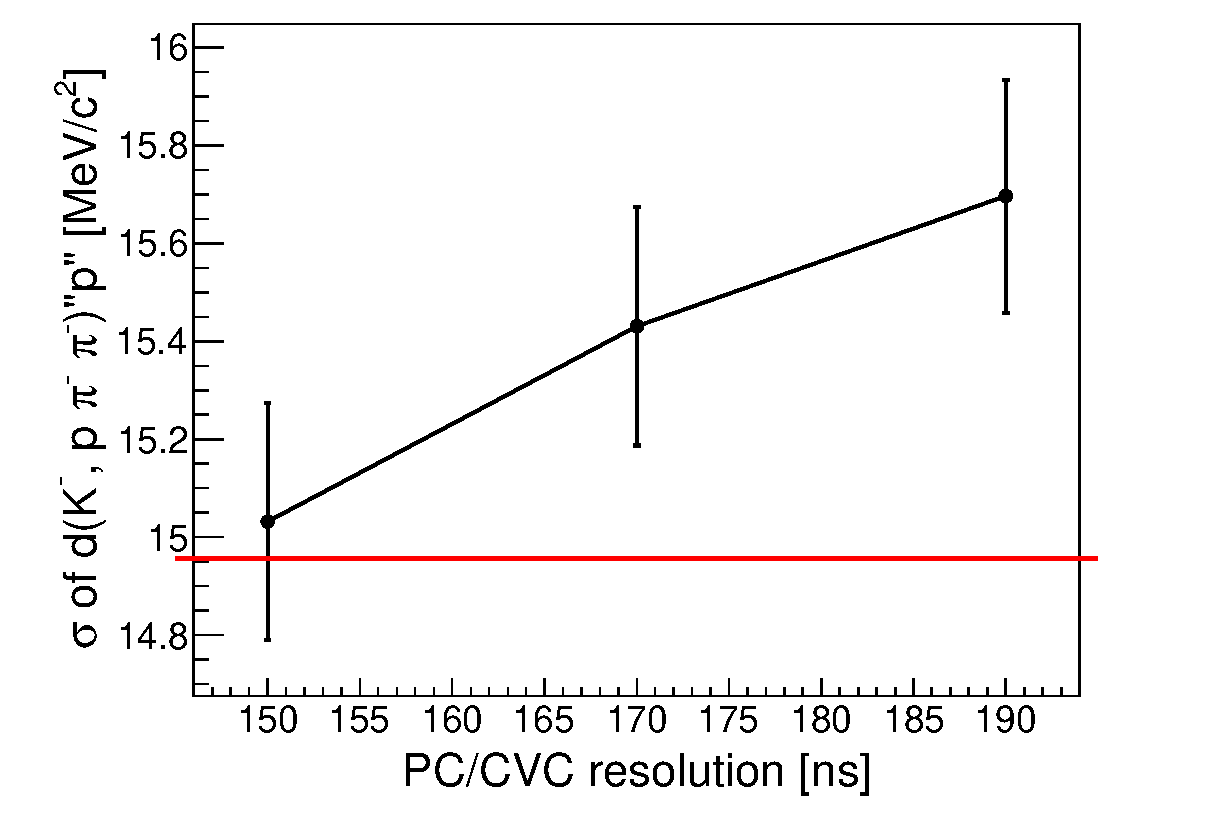
\includegraphics[width=7cm]{../pic/Dron/FP_reso.eps}
    \end{minipage}
  \end{tabular}
  \caption{
    Left figure shows $d(K^-, p \pi^- \pi^-)"p"$ missing mass spectrum in $d(K^-, p)"\pi^-\Lambda"$ events.
    Red line indicates fitting result.
    Right figure indicates relation of $\sigma$ of $d(K^-, p \pi^- \pi^-)"p"$ peak which was estimated Gaussian fitting and inputed time resolution.
    Red line indicate fitting result of the data.
  }
  \label{fig:FP_reso}
\end{figure}

\begin{figure}[htbp]
  \centering
  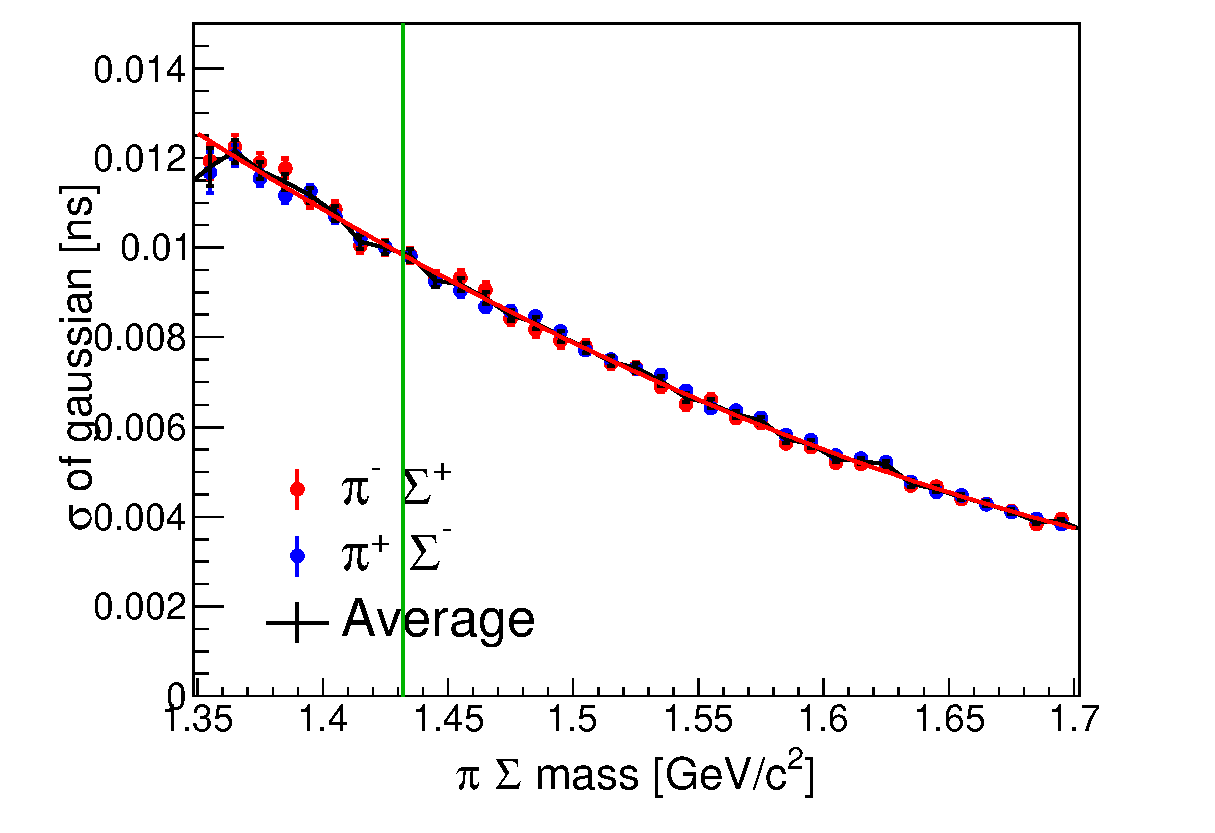
\includegraphics[width=8cm]{../pic/Dron/NC_reso_KN_MM_NC170.eps}
  \caption{
    This figure indicates about $d(K^-, n)"X"$ missing mass resolution which was estimated by the $d(K^-, n)"\pi^{\mp}\Sigma^{\pm}"$ Monte Carlo simulation.
    Red, blue and black plot indicates the $d(K^-, n)"\pi^-\Sigma^+"$, the $d(K^-, n)"\pi^+\Sigma^-"$ and average of these, respectively.
    Fitted 3rd polynomial function is plotted at same time.
  }
  \label{fig:KN_MM_reso}
\end{figure}
